\part{Analysis}
\textit{Results from the implementation}
%present the details of the experiments
%   i. Hardware and Software info
%  ii. NN implementations : challenges in developing model & build for target HW
% iii. Different performance measurements: Training time, Model accuracy, Peak 	%	   memory utilised and memory footprint
%  iv. 
A hand digit recognition neural network (HDR-NN) model is implementated in C, C++ Eigen, Python Numpy and Pytorch. The performance of HDR-NN training implementations was evaluated on the iMX6SDB evaluation board, which was programmed with an Embedded Linux built using The Yocto Project. To gauge the effectiveness of the models, we compared model accuracy, execution time, and peak memory usage while altering the number of layers and neurons in each layer. Furthermore, we address the obstacles encountered in developing the NN model and compiling it to operate on the target hardware. 

%Ideas: 1. Coefficient of variation
%		2. optimisation flags
%		3. Measurements using different tools 
%		4. Early stopping
%		5. Choosing Model parameters
%		6. Extrapolation

\chapter{Results}
The HDR-NN models implemented in all paradigms have a constant input size of 784 and output size of 10. The hidden layer sizes vary depending on the implementation:
\begin{itemize}
	\item C and C++ Eigen: 2, 4, 8, 32, 128, (32,16), and (128,16)
	\item Python-Numpy: 2, 8, 32, (32,16)
	\item Tensorflow/Pytorch:
\end{itemize}
The model implemented is a fully connected neural network with stocastic gradient descent and mean square error. The biases and wieghts are randomly initialised using the same random generator and initial seed. The hyperparameters   
The model accuracy, training time, and peak memory usage are measured for each implementation and all its hidden layer settings. This experiment is repeated 10 times and the final values are the average of all iterations.
% feedforward NN with backpropogation for updating gradients
% dataset mnist
% epochs = 30;
% batchSize = 10;
% eta = 3;
% sigmoid activation 
% unoptimised code with scope for futher improvement

% hardware Cortex A9 processor with armv7 architecture
% board supports dual/quad core but implementations use single core to train the models
% fpu support
% data structures used by different implementations
% yocto image with fsl-imx-linux distro, zImage and ext4 file system
% embedded linux size a average size of 500Mb with core-image-base image recipe. 

% perf and GNU time tools for measurements. 10 runs atleast for each configuration of hidden layer size


\section{Accuracy}
The different implementation perform similarly in model accuracy. This is expected as the models have the exact structure and configurations.  
\begin{figure}[ht]
	\centering
	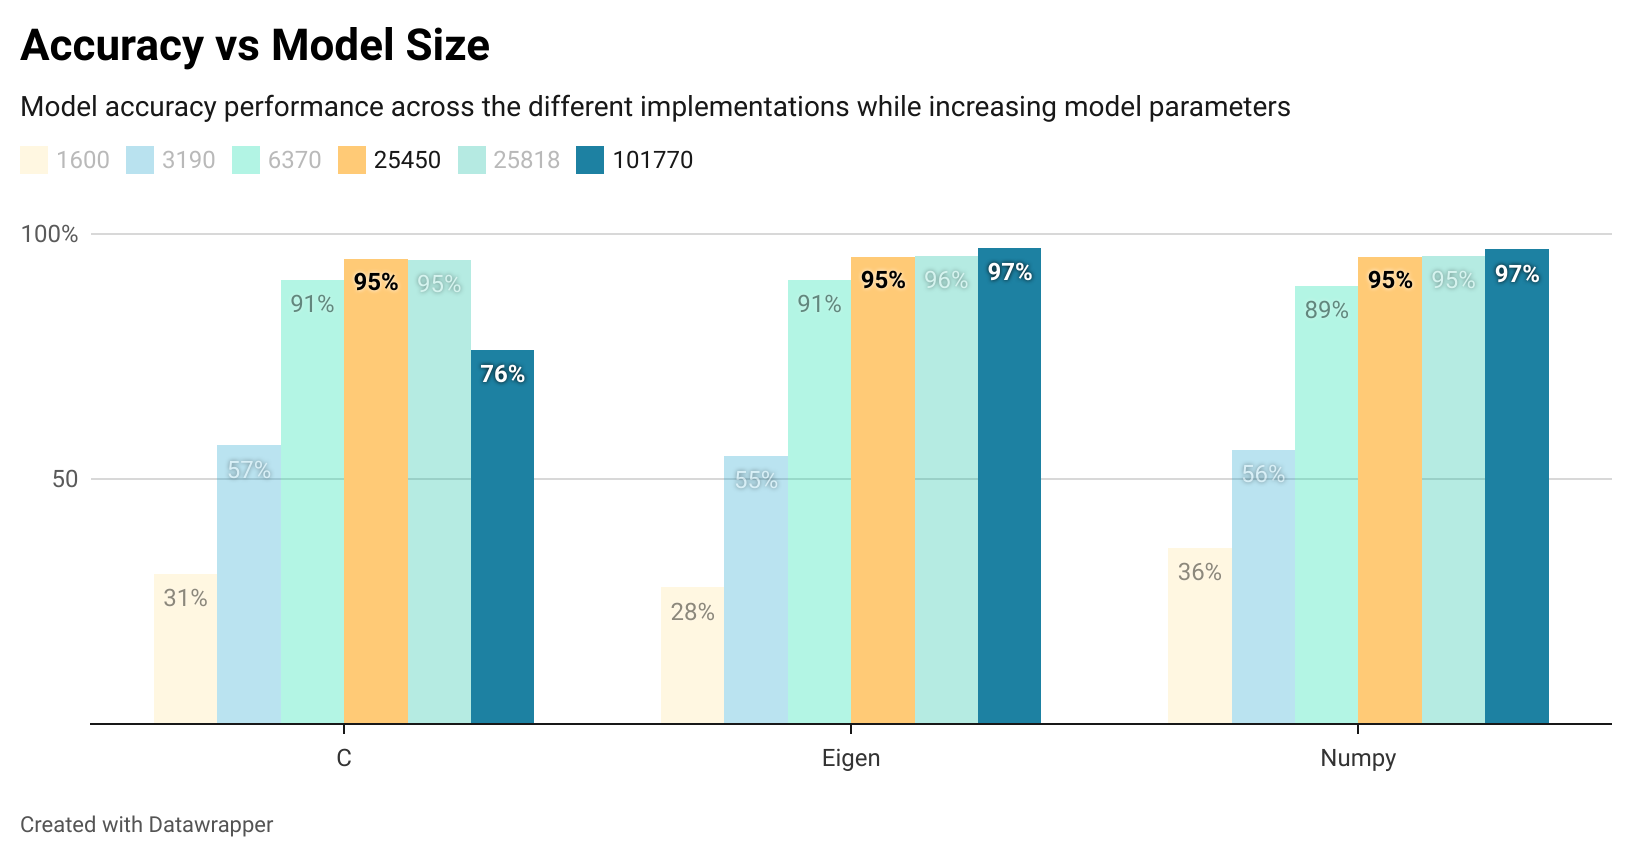
\includegraphics[scale=0.37]{accuracy}
	\caption[HDR-NN Accuracy]{Comparing the accuracy of the different HDR-NN implementations.}
\end{figure}

Further, when the number of neurons in a single layer exceeds 32, the accuracy of the model is observed to decrease due to overfitting. To improve accuracy, adding another layer with 16 neurons is found to be beneficial without significantly increasing the time required for computation. In fact, for larger network sizes, it is observed to even reduce the computation time required.


\section{Execution Time}
The run times increased exponentially with the number of parameters. This is due to the fact that the amount of calculation in a fully connected network increases with the number of neurons, leading to longer training times

\begin{figure}[ht]
	\centering
	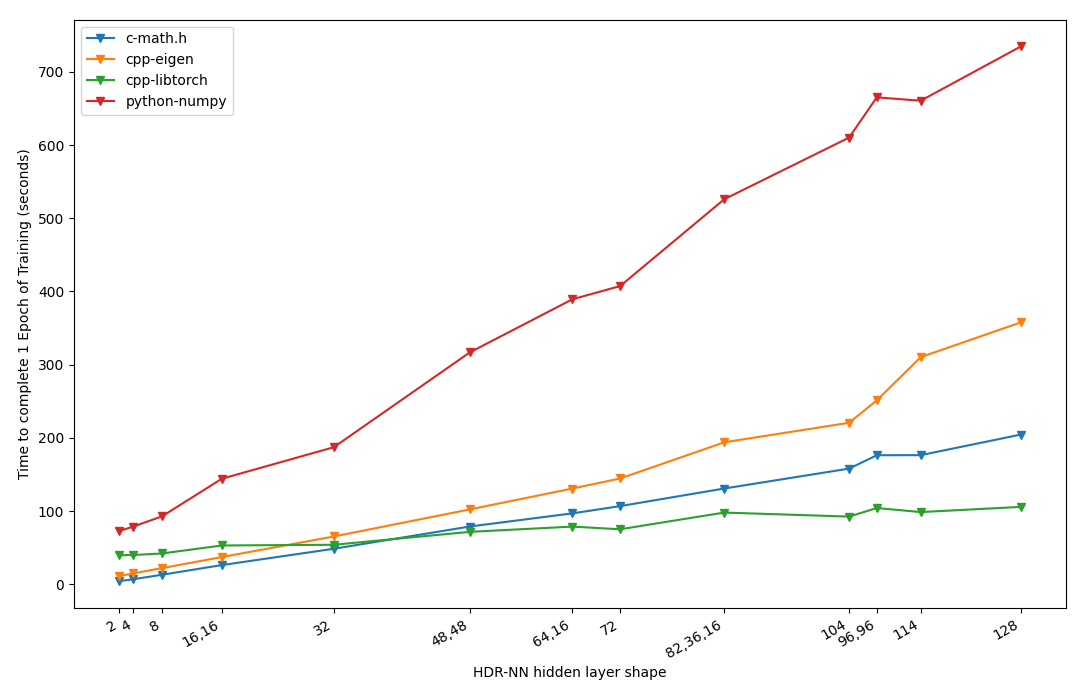
\includegraphics[scale=0.35]{exec-time}
	\caption[Execution Time vs Model Parameters]{Comparing total run time for training the different HDR-NN programs}
\end{figure}

\section{Peak Memory Usage}
Regardless of the hidden layer sizes, the peak memory utilisation remains constant for the same application regardless of the network configuration. C++ Eigen implementation has the least run time memory footprint while Python Numpy is the worse performing. 
\begin{figure}[ht]
	\centering
	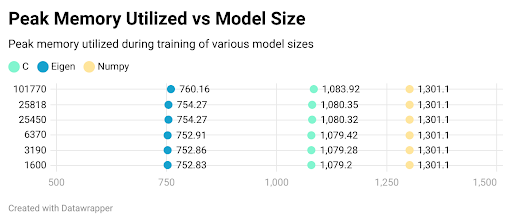
\includegraphics[scale=0.31]{memory-bar}
	\caption[Peak Memory Utilisation]{Peak Memory Utilized during training with different model sizes remain similar within the same implementation}
\end{figure}


\subsection[Python - Numpy]{Python Numpy based HDR-NN}

The Numpy implementation consistantly took longer duration to perform the same training cycle as compared to the C implementation

\subsection[Tensorflow Lite]{Tensorflow-Lite based HDR-NN}
\textit{Benchmark pending \dots}

\subsection[C]{C based HDR-NN}

C implementation had lower execution times and memory usage

\subsection[CPP - Eigen]{CPP based HDR-NN}
\textit{Benchmark pending \dots}

\section{CMSIS-NN based Optimisations to Training}
\textit{Further breakdown of the performance achieved from different optimisation techniques}

\subsection{Quantisation}
\textit{future: Training Network with Quantized weights}

\subsection{Pruning the Network}
\textit{future}

\section{Coefficient of variation}
A total of 10 iterations were conducted to ensure that the results remained consistent. To assess the degree of variability among the various trials, the mean and standard deviation were calculated across all runs, and their ratio was determined. This ratio indicates the level of variation between the different tests.

\chapter{Discussion}

\begin{itemize}
	\item \textit{Contrast development process for the ML programming paradigms}
	\item \textit{Which optimisation approaches gave the most in improvement?}
\end{itemize}

\section{Early stopping}
The training for all the implementations were executed by configuring the number of epochs as 30. This leads to the accuracy of model dropping significantly due to overfitting, which could be avoided if early stopping was implemented.
But, early stopping is not implemented as the performance would be completely different and there wouldn't be a standard setting to compare the implementations.



\chapter{Conclusion and Future Work}
\textit{What does it all mean? Where do we go from here?}
